\chapter{Formatting options}\label{ch:introduction}

The best way to view this document is in a split-view format, with the \texttt{.tex} file open and the corresponding portion of the \texttt{.pdf} output also visible.

\section{Equations and tables}\label{sec:equationexamples}

You can write an equation without a label by using an asterisk:
\begin{equation*}
f(x) = (x+a)(x+b).
\end{equation*}
Alternatively, you can number and label your mathematical expressions:
\begin{equation}\label{eq:Lagrangian_EM}
\mathcal{L}_{\text{EM}} 
  = \frac{1}{2} \biggl( \epsilon_{0} \left| \vect{E} \right|^{2} + \frac{1}{\mu_{0}} \left| \vect{B} \right|^{2} \biggr)
   - \phi \varrho_{\text{free}} + \vect{A} \cdot \vect{J}_{\text{free}}
   + \vect{E} \cdot \vect{P} + \vect{B} \cdot \vect{M}.
% = \mathcal{L}_{\text{field}} + \mathcal{L}_{\text{int}}
% = - \frac{1}{4 \mu_{0}} F^{\alpha \beta} F_{\alpha \beta} - A_{\alpha} J^{\alpha}.
\end{equation}
This way, we can later reference something we wrote earlier, like the electromagnetic Lagrangian density in non-relativistic vector notation shown in Equation (\ref{eq:Lagrangian_EM}).\\

The equation environment allows you to construct a number of objects, such as arrays and algined sets of equations. For instance, we might want to write a general matrix:
\begin{equation}
\vect{c} = 
  \left(\begin{array}{c c c c c}
    c_{11} & c_{12} & c_{13} & \ldots & c_{1n} \\
    c_{21} & c_{22} & c_{23} & \ldots & c_{2n} \\
    c_{31} & c_{32} & c_{33} & \ldots & c_{3n} \\
    \vdots & \vdots & \vdots & \ddots & \vdots \\
    c_{m1} & c_{m2} & c_{m3} & \ldots & c_{mn} \\
  \end{array}\right).
\end{equation}
We might alternatively want to write a set of simultaneous equations. If future descriptions require for all of them to have unique labels, try using the `subequations' environment as well as the `eqnarray' environment.
\begin{subequations}\label{eq:simulALL}
\begin{eqnarray}
 3x + 5y +  z &=& 5\\ \label{eq:simulB}
 7x - 2y + 4z &=& 3\\
-6x + 3y + 2z &=& 1.
\end{eqnarray}
\end{subequations}
This will allow you to talk about the set of simultaneous equations as a whole by referring the reader to Equation (\ref{eq:simulALL}), or else to a specific statement like Equation (\ref{eq:simulB}).\\

Sometimes you'll want to derive a result, which in its clearest form requires more than one line of algebra. There are a few ways to accomplish this, and the best choice will depend on the task at hand and your personal taste. You can instruct the compiler \textit{not} to give a label to one or more of the lines as you go.
\begin{eqnarray}\notag
\lefteqn{R_{x} (\varepsilon) R_{y} (\varepsilon) - R_{y} (\varepsilon) R_{x} (\varepsilon)} \\ \notag
& = &  \left( 1 - \frac{i J_{x} \varepsilon}{\hbar} - \frac{J_{x}^{2} \varepsilon^{2}}{2 \hbar^{2}} \right) 
 \left( 1 - \frac{i J_{y} \varepsilon}{\hbar} - \frac{J_{y}^{2} \varepsilon^{2}}{2 \hbar^{2}} \right) - 
 \left( 1 - \frac{i J_{y} \varepsilon}{\hbar} - \frac{J_{y}^{2} \varepsilon^{2}}{2 \hbar^{2}} \right)
 \left( 1 - \frac{i J_{x} \varepsilon}{\hbar} - \frac{J_{x}^{2} \varepsilon^{2}}{2 \hbar^{2}} \right) \\
& = &  \left( 1 - \frac{i J_{z} \varepsilon^{2}}{\hbar} \right) - 1 + \mathcal{O} (\varepsilon^{3}). 
\end{eqnarray}

A table of data is sometimes necessary, for which there is a dedicated environment. An example of this is given in Table (\ref{tab:measuredconstants}) -- note that the counter for tables is separate from the counter for equations. If this isn't to your liking, you can change the enumeration style of one or both. (Google has plenty of suggestions).

\begin{table}[h!]
\begin{center}
\begin{tabular}{ l l l c l}\hline
\textbf{description}  & \textbf{} & \textbf{value} \\ \hline
electronic charge & $e$ & $1.6021766 \times 10^{-19} \coulomb$ \\
proton mass            & $m_{p}$ & $1.6726218 \times 10^{-27} \kilo\gram$ &  
 or & $938.27203 \mega\electronvolt\per c^{2}$ \\
electron mass          & $m_{e}$ & $9.1093822 \times 10^{-31} \kilo\gram$ & or & $510.99891 \kilo\electronvolt\per c^{2}$ \\
permittivity of vacuum & $\epsilon_{0}$ & $8.8541878 \times 10^{-12} \farad\per\meter $ \\
permeability of vacuum & $\mu_{0}$         & $1.2566371 \times 10^{-6} \; \henry\per\meter$ & 
 or & $4 \pi \times 10^{-7} \henry\per\meter $ \\
speed of light in vacuum & $c$               & $2.9979246 \times 10^{+8} \; \meter\per\second $ \\ 
electrostatic constant   & $k_{e}$ & $8.9875518 \times 10^{+9} \; \meter\per\farad$ & 
 or & $1/4 \pi \epsilon_{0}$ \\
Planck constant        & $h$ & $6.6260696 \times 10^{-34} \; \joule\cdot\second$ & 
 or & $4.1356675 \times 10^{-15} \electronvolt\cdot\second$ \\
reduced Planck constant        & $\hbar$ & $1.0545717 \times 10^{-34} \; \joule\cdot\second$ & 
 or & $6.5821193 \times 10^{-16} \electronvolt\cdot\second$ \\
\hline
\end{tabular}
\end{center}
\caption{A table of measured constants.}
\label{tab:measuredconstants}
\end{table}

\section{Pictures and figures}\label{sec:figures}
Try to stick to a few data formats if possible. Vector and pdf data types are ideal, because they minimise the overall size of the document and you can zoom/print to any quality without pixelisation.\\

You can write a program that returns data or a visual representation of it (graph, coloured array, surface plot etc.), and in the latter case, you can take the resulting image and copy to your `figures' folder (this keeps the internal address conventions neat and tidy) and link the document directly to your report, like so:\\

\begin{figure}[h!]
\begin{center}
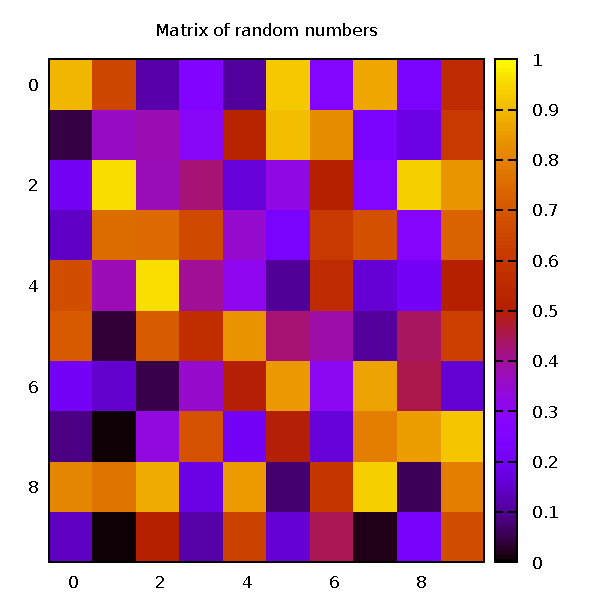
\includegraphics[width=0.40\linewidth]{figures/random_matrix.pdf}
\end{center}
\caption{A random square matrix, generated by a \texttt{Fortran} program.}
\label{fig:random_matrix}
\end{figure} 


If you need to provide a diagram of your own creation, there are several options available. You can feel free to choose whichever method your experience has endowed you with, or else represents the best compromise between effort spent and professional appearance of the final product. For instance, you could hand-draw your diagram, scan or take a photo of it, upload the resulting image to the correct directory, crop/filter it and add to your document, as shown in the LHS of Figure (\ref{fig:handcomp}).\\

Alternatively, you could use some available computer software to get the job done. Here we will give you an example made in Inkscape, because it is an open-source package which is available for most operating systems. Here you will make your diagram (there are plenty of tutorials and examples available online), adjust the document borders to your satisfaction, save a vector-type copy for later editing purposes (for instance, `\texttt{diagram.svg}', and then also save a pdf version (`\texttt{diagram.pdf}'). It is the second file-type which you can link to your \LaTeX document with the usual features. The comparison between a hand-drawn and computer-rendered image is fairly stark -- see the RHS of Figure (\ref{fig:handcomp}).\\

\begin{figure}[h!]
\begin{center}
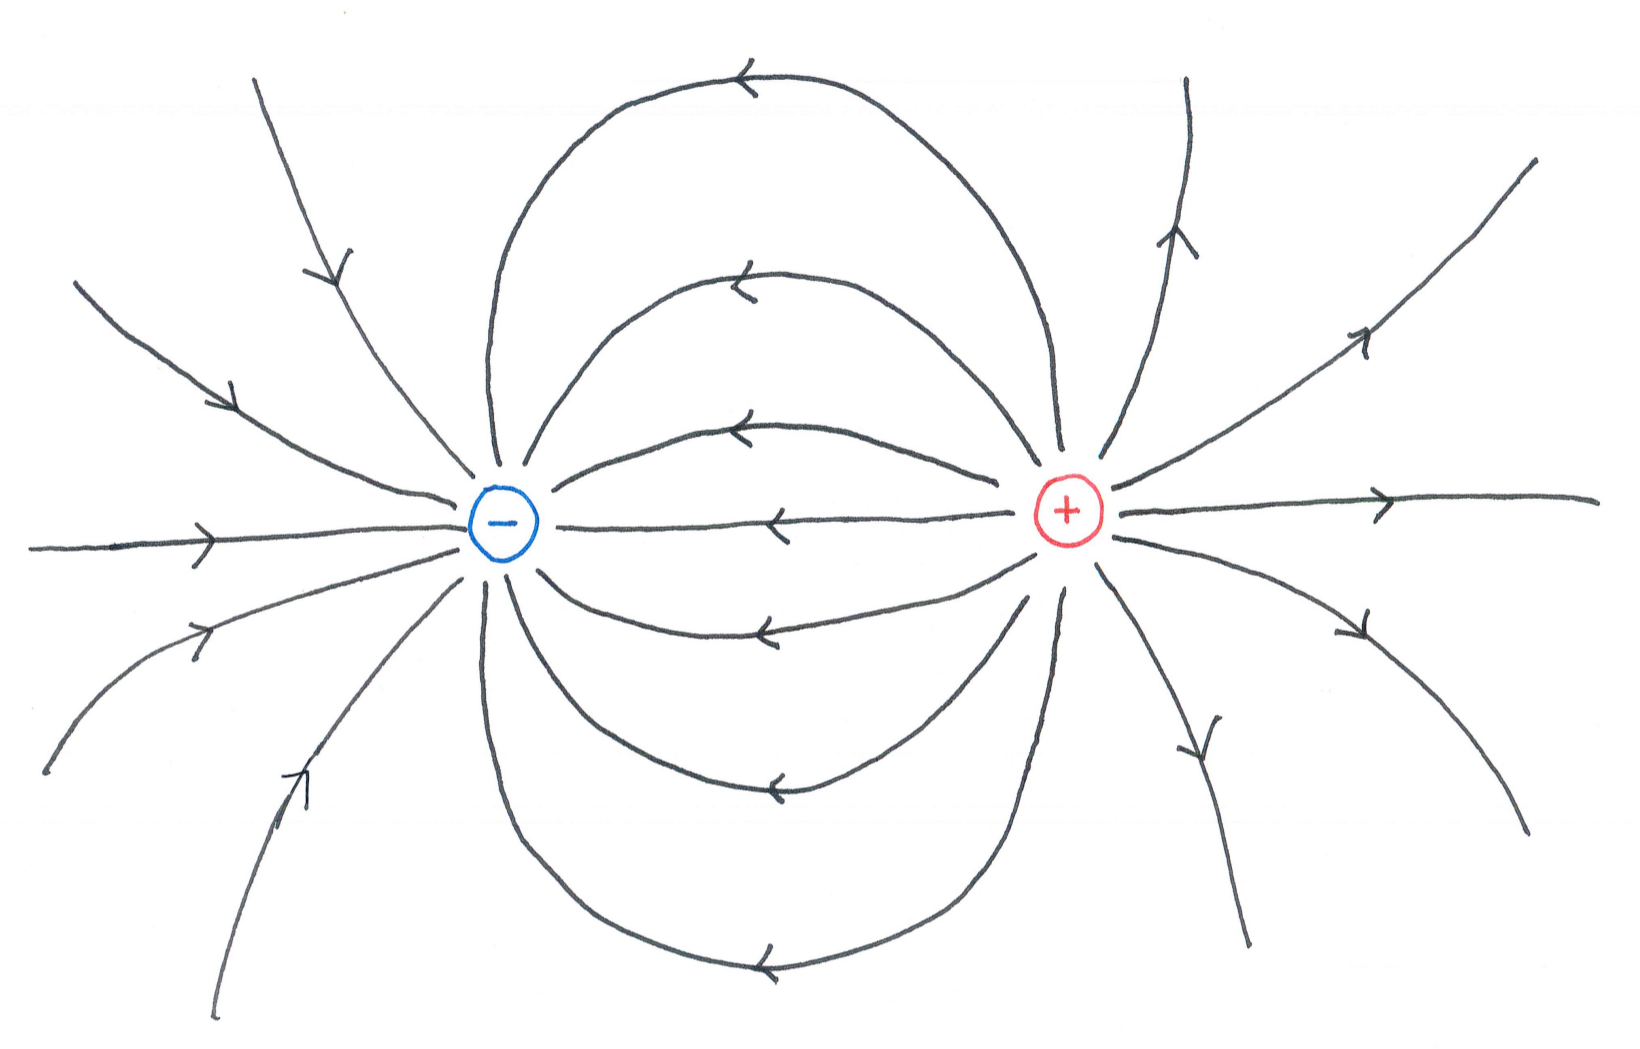
\includegraphics[width=0.50\linewidth]{figures/dipole_hand.png}\hspace{1cm}
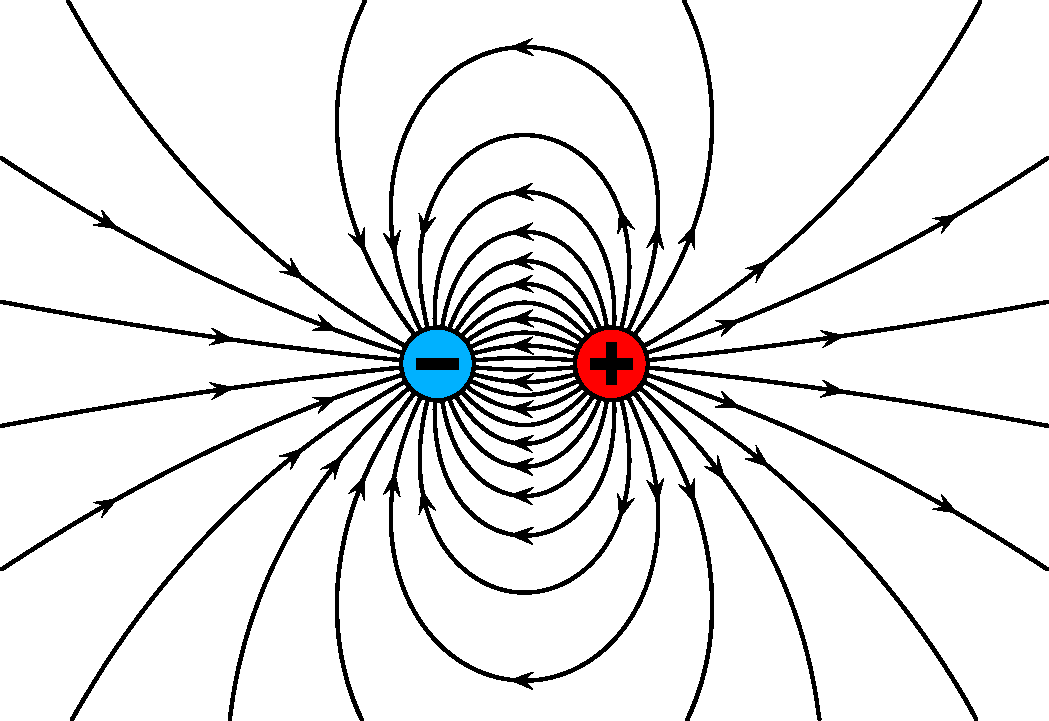
\includegraphics[width=0.40\linewidth]{figures/dipole_vector.pdf}
\end{center}
\caption{A sketch of some electric field lines around an ideal electric dipole.}
\label{fig:handcomp}
\end{figure}

If you wish to take the last example further, try exploring some of Inkscape's features. It allows you to plot functions, write mathematical expressions (although this option does not always work) and vectorise/edit a surprisingly large assortment of existing images. If you would like your final document to look seamlessly consistent, you can even make diagrams with text and equations of the same formatting. (This involves writing everything in a dummy \LaTeX document, exporting and vectorising it online, importing that vector document into Inkscape, playing around with character size compared to final drawing size in the document, and then exporting that diagram as a pdf to be placed back into \LaTeX ... possibly not a worthwhile pursuit for the purposes of this subject.)

\section{Computer code}\label{sec:code}
\subsection{Code input/output}\label{subsec:codeinout}

Talk about the language that you used, maybe referencing an integral in \cite{abramowitz1970} or a numerical algorithm in \cite{press1992} if you used \texttt{Fortran}.

\subsection{Code written verbatim}\label{subsec:verbatim}

This can be done with the \texttt{listings} and \texttt{verbatim} packages. You should modify the preamble document so that these packages correctly interpret the programming language that you used.

\newpage

\begin{lstlisting}
      FUNCTION PINEWT(N)
      IMPLICIT DOUBLE PRECISION (A-H,O-Z)
C**********************************************************************C
C     PINEWT EVALUATES THE INFINITE SERIES REPRESENTATION              C
C     FOR PI AS A TRUNCATED SUM.                                       C
C**********************************************************************C
C
C     ENSURE N IS A LEGAL VALUE
      IF(N.LT.0) THEN
        WRITE(6,*) 'In PINEWT: illegal value for N.',N
        RETURN
      ELSEIF(N.EQ.0) THEN
        PINEWT = 2.0D0
      ENDIF
C
C     INITIALISE SOME COUNTERS
      TWOPOW = 1.0D0
      FACKNM = 1.0D0
      FACKDM = 1.0D0
      PINEWT = TWOPOW*FACKNM*FACKNM/FACKDM
C
C     LOOP OVER SERIES ORDER N TIMES, ADDING EACH TERM TO TOTAL
      DO I=1,N
        TWOPOW = 2.0D0*TWOPOW
        FACKNM = DFLOAT(I)*FACKNM
        FACKDM = DFLOAT(2*I+1)*DFLOAT(2*I)*FACKDM
        PINEWT = PINEWT + TWOPOW*FACKNM*FACKNM/FACKDM
      ENDDO
C
C     DOUBLE THE RESULT (SEE WIKIPEDIA FORMULA)
      PINEWT = 2.0D0*PINEWT
C
      RETURN
      END
\end{lstlisting}